\documentclass{article}
\usepackage[utf8]{inputenc}
\usepackage[T1]{fontenc}
\usepackage{amsmath}
\usepackage{tikz}
\usetikzlibrary{shapes.geometric, arrows}
\usetikzlibrary{shapes}
\usetikzlibrary{positioning}
\usetikzlibrary{fit}
\usetikzlibrary{shadows}
\usetikzlibrary{calc}
\usetikzlibrary{decorations.markings}
\usetikzlibrary{arrows.meta, bending, intersections}
\tikzset{splrect/.style = {rectangle split, rectangle split horizontal,
                           rectangle split parts=5, minimum height=1cm, 
                           align=center, draw=black},
         rect/.style = {rectangle, rounded corners, minimum width=3cm,
                        minimum height=1cm,text centered, text width=3cm,
                        draw=black},
         rect2/.style = {rectangle, rounded corners, minimum width=4cm,
                        minimum height=1cm,text centered, text width=4cm,
                        draw=black},
         redrect/.style = {rectangle, rounded corners, minimum width=3cm,
                           minimum height=1cm,text centered, text width=3cm,
                           draw=black, fill=red, fill opacity=0.5},%
         freerect/.style = {rectangle, rounded corners, minimum width=10cm, minimum height=1cm, draw=black, text centered, text width=10cm},
         arrow/.style = {->,shorten >=1pt,>=stealth',semithick},
         labl/.style = {minimum width=3cm,
                        minimum height=1cm,text centered, text width=3cm,
                        draw=black!0},
         doc/.style={draw, minimum height=4em, minimum width=3em, text width=3cm, text centered, fill=white, double copy shadow={shadow xshift=4pt, shadow yshift=4pt, fill=white, draw}},
         decision/.style={diamond, minimum width=3cm, minimum height=1cm, text centered, draw=black}
}
\tikzset{
  invisible/.style={opacity=0},
  visible on/.style={alt={#1{}{invisible}}},
  alt/.code args={<#1>#2#3}{%
    \alt<#1>{\pgfkeysalso{#2}}{\pgfkeysalso{#3}}
  },
}

\begin{document}

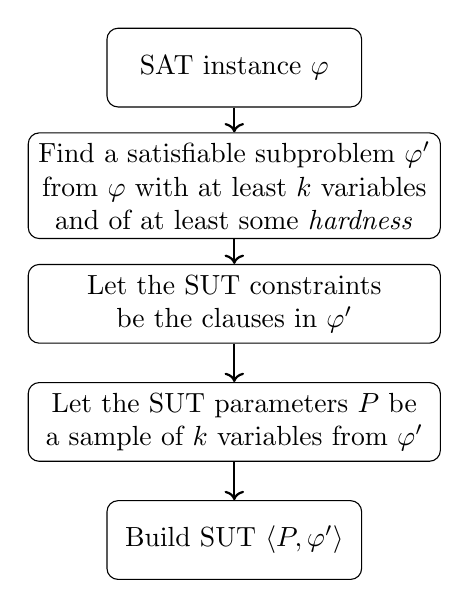
\begin{tikzpicture}[node distance=1.5cm]
    \node (n1) [rect] {SAT instance $\varphi$};
    \node (n2) [rect, text width=5cm, below of = n1] {Find a satisfiable subproblem $\varphi'$ from $\varphi$ with at least $k$ variables and of at least some \emph{hardness}};
    \node (n3) [rect, text width=5cm, below of = n2] {Let the SUT constraints be the clauses in $\varphi'$};
    \node (n4) [rect, text width=5cm, below of = n3] {Let the SUT parameters $P$ be a sample of $k$ variables from $\varphi'$};
    \node (n5) [rect, below of = n4] {Build SUT $\langle P, \varphi' \rangle$};
    
    \draw [->, thick] (n1) -- (n2);
    \draw [->, thick] (n2) -- (n3);
    \draw [->, thick] (n3) -- (n4);
    \draw [->, thick] (n4) -- (n5);
\end{tikzpicture}

\end{document}